\chapter{Theory and Key Concepts}

\section*{Introduction}
In this chapter, we will explore the key concepts essential to our project. We begin by introducing the STM32 ecosystem, providing an overview of its components and their functionalities. Following this, we delve into the theoretical aspects of benchmarking and embedded build systems relevant to our work. Finally, we will discuss the essentials of automating project generation.



\section{STM32 Microcontrollers (MCUs)}
\subsection{STM32 Series}
STM32 microcontrollers (MCUs) are a family of 32-bit microcontrollers based on the ARM Cortex-M processor. Developed by STMicroelectronics, the STM32 series offers a wide range of products that cater to various applications, from simple embedded systems to complex industrial automation.
The STM32 MCUs are categorized into several series, each designed to meet specific application requirements. Some of the most commonly used series are the \textbf{STM32F} series and the \textbf{STM32H} series. Within each series.
\subsection{ARM Cortex-M}
The STM32 microcontrollers are built around the ARM Cortex-M cores, which are designed for efficient and high-performance processing in embedded systems. 
The ARM Cortex-M family includes several cores, such as Cortex-M0, Cortex-M4, Cortex-M7, and Cortex-M85, each offering different levels of performance and features.

STM32 MCUs are grouped into families, a combination of a series and an ARM Cortex-M core, the number proceeding the STM32 series indicates the core, for example, STM32H7 family indicates a microcontroller from the STM32H series with a Cortex-M7 core, while the STM32N6 family indicates a STM32N series microcontroller with a Cortex-M55 core. 
\subsection{STM32 UART Peripheral}
STM32 microcontrollers come with a rich set of integrated peripherals (IPs) that enhance their functionality and enable developers to build complex and feature-rich applications. The one of interest in this report is the UART peripheral.
UART is a hardware protocol and communication interface that uses two wires for data exchanges between peripherals that do not share a common clock signal. It fits our use case of transmitting data from the microcontroller to the host computer in order to have access to Coremark results.
\newpage
\subsection{STM32Cube Firmware Package}
The STM32Cube Firmware Package is a comprehensive software suite provided by STMicroelectronics to accelerate development on STM32 microcontrollers. Its components include but are not limited to:
\begin{itemize}
    \item \textbf{CMSIS:} A vendor-independent standard defined by Arm that provides a consistent API for Cortex-M cores, STM32Cube Firmware provides an implementation of the CMSIS-Core layer, these include device and family specific header files, as well as templates for startup files and linker scripts.
    \item \textbf{HAL:} Simplifies peripheral configuration and access through high-level APIs, reducing development complexity and allows for re-usability across different hardware.
    \item \textbf{LL Drivers:} Provide fine-grained control of peripherals with minimal overhead, suitable for performance-critical applications.
\end{itemize}

Together, these components create an environment where developers can choose the appropriate level of abstraction based on their specific requirements, all while maintaining compatibility and code re-usability across the STM32 ecosystem.


\section{Benchmarking}
\subsection{Overview}
Benchmarking is the systematic process of evaluating and comparing the performance of a computing system, or a specific component within that system, by running a standardized set of tasks and synthetic workloads.
The key aspects of benchmarks include:
\begin{itemize}
    \item \textbf{Metrics:} Performance is measured using quantifiable units, Common metrics include:
        \begin{itemize}
            \item \textbf{Throughput:} The amount of work done per unit of time (e.g., operations/second, frames/second, MB/s).
            \item \textbf{Latency:} The time taken to complete a single operation (e.g., microseconds per operation).
            \item \textbf{Power Efficiency:} Performance achieved per watt of power consumed (e.g., points per watt, inferences per joule).
            \item \textbf{Memory Usage:} The amount of RAM or cache consumed during a task.
            \end{itemize}
    \begin{samepage}
    \item \textbf{Benchmark Types:}
        \begin{itemize}
            \item \textbf{Synthetic Benchmarks:} These are specialized programs designed to stress specific subsystems like the CPU, memory, or GPU. They provide standardized but often abstract results.
            \item \textbf{Application Benchmarks:} Use real-world software and workloads (e.g., rendering a video file, compiling a large code-base, running a specific game at a set quality). These measure performance in practical, user-facing scenarios.
            \item \textbf{Micro-benchmarks:} Isolate and test a very specific, low-level operation (e.g., floating-point multiplication speed, memory access latency).
        \end{itemize}
    \end{samepage}
\end{itemize}
\subsection{Benchmarking Microcontrollers}
Although the same benchmarks can be run on most pieces of technology, the implementation differs slightly for microcontrollers. Computers can delegate tasks such as scheduling and printing to the underlying operating system, which is not the case when it comes to embedded devices. We have to take into account handling threads, I/O operations, memory regions, and code sections. This can make the implementation tricky at times.
The following steps are necessary to ensure proper benchmarking on a microcontroller:
\begin{itemize}
    \item \textbf{Clock Source Provision:} Benchmarks rely on CPU ticks in order to get an accurate estimate of the time taken to run the workloads, providing access to the tick counter, whether it be the internal System Clock or an external timer, as well as the frequency of said clock is crucial for proper measurements.
    \item \textbf{Print Logic Implementation:} Computers can offer multiple ways of getting data from a program, such as logging them into files or printing them to the standard output, this option is not available on microcontrollers, therefore, we have to provide our own mechanism of data transmission. In our context, the print logic was implemented to send data via the UART peripheral.  
    \item \textbf{Code Execution Management:} For high-end systems relying on an operating system, the most common approach is to load the program from disk into volatile memory(RAM) and begin execution without any extra steps. However, in our case, we have to specify the regions of memory where each part of the program will reside, the most common types of memory are: FLASH, SRAM, ITCM/DTCM, SDRAM, NVMe, all of them can be either external or internal. Depending on multiple factors, such as wait-states, clock synchronization and the communication interface, the results can have vastly varying results depending on the chosen regions.
\end{itemize}
\subsection{Coremark}
There have been many attempts to provide a single number that can totally quantify the
ability of a CPU. Be it MHz, MOPS, MFLOPS - all are simple to derive but misleading
when looking at actual performance potential.
EEMBC’s CoreMark is a benchmark that measures the performance of microcontrollers (MCUs) and central processing units (CPUs) used in embedded systems.
It is designed to run on devices from 8-bit microcontrollers to 64-bit microprocessors.
CoreMark ties a performance indicator to execution of simple
code, but rather than being entirely arbitrary and synthetic, the code for the benchmark
uses basic data structures and algorithms that are common in practically any application
\subsubsection*{Coremark Composition}
To appreciate the value of CoreMark, it’s worthwhile to dissect its composition, which in
general is comprised of lists, strings, and arrays (matrixes to be exact). Lists commonly
exercise pointers and are also characterized by non-serial memory access patterns. In
terms of testing the core of a CPU, list processing predominantly tests how fast data can
be used to scan through the list. For lists larger then the CPU’s available cache, list
processing can also test the efficiency of cache and memory hierarchy.
\subsubsection{List Processing}
List processing consists of reversing, searching or sorting the list according to different
parameters, based on the contents of the list data items. In particular, each list item can
either contain a pre-computed value or a directive to invoke a specific algorithm with
specific data to provide a value during sorting. To verify correct operation, CoreMark
performs a 16b cyclic redundancy check (CRC) based on the data contained in elements
of the list. Since CRC is also a commonly used function in embedded applications, this
calculation is included in the timed portion of the CoreMark.
\subsubsection{Matrix Processing}
Many algorithms use matrixes and arrays, warranting significant research on optimizing
this type of processing. These algorithms test the efficiency of tight loop operations as
well as the ability of the CPU and associated toolchain to use ISA accelerators such as
MAC units and SIMD instructions. These algorithms are composed of tight loops that
iterate over the whole matrix. CoreMark performs simple operations on the input
matrixes, including multiplication with a constant, a vector, or another matrix. CoreMark
also tests operating on part of the data in the matrix in the form of extracting bits from
each matrix item for operations. To validate that all operations have been performed,
CoreMark again computes a CRC on the results from the matrix test.
\subsubsection{State machine processing}
An important function of a CPU core is the ability to handle control statements other than
loops. A state machine based on switch or ‘if’ statements is an ideal candidate for testing
that capability. There are 2 common methods for state machines – using switch
statements or using a state transition table. Because CoreMark already utilizes the latter
method in the list processing algorithm to test load/store behavior, CoreMark uses the
former method, switch and ‘if’ statements, to exercise the CPU control structure.
The state machine tests an input string to detect if the input is a number, if it is not a
number it will reach the “invalid” state. This is a simple state machine with 9 states. The
input is a stream of bytes, initialized to ensure we pass all available states, based on an
input that is not available at compile time. The entire input buffer is scanned with this
state machine.
\subsubsection{CoreMark Profiling}
Since CoreMark contains multiple algorithms, it is interesting to demonstrate how the
behavior changes over time. For example, looking at the percentage of control code
executed (samples taken at each 1000 cycles) and branch mis-predictions in Figure \ref{fig:coremark_control}, it is
obvious where the matrix algorithm is being called. This is portrayed by the low mis-
prediction rate and high percentage of control operations, indicative of tight loops) (for example,
between points 330-390).
\begin{figure}[H]
  \centering
  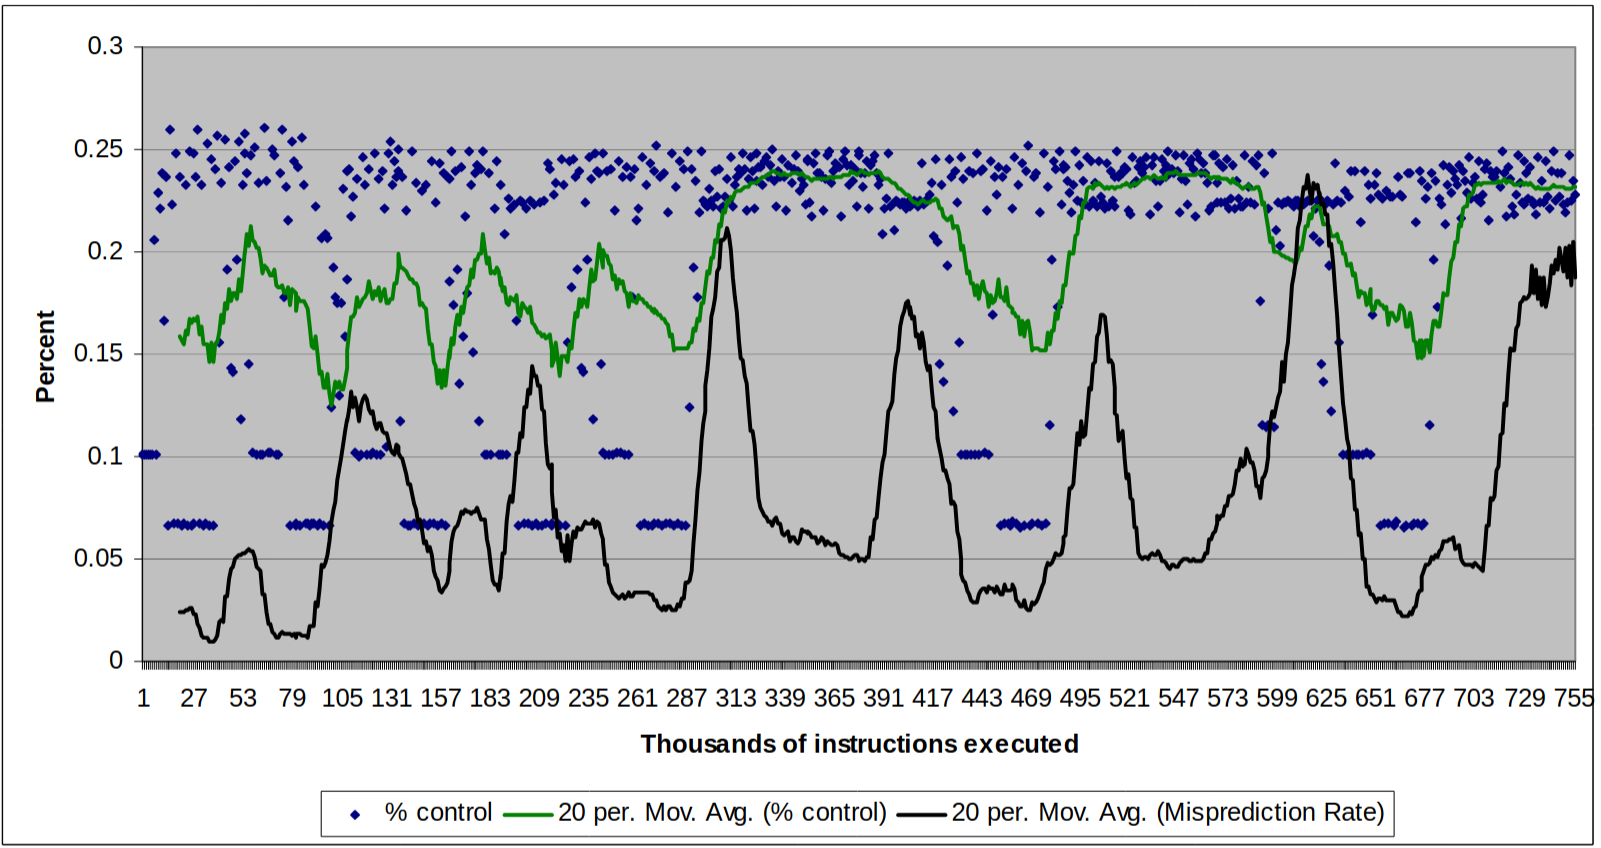
\includegraphics[width=15cm]{img/ST_Summer_Internship/coremark_control_instructions.png}
  \caption{Distribution of control instructions and mispredictions over CoreMark execution.}
  \label{fig:coremark_control}
\end{figure}

Overall CoreMark is well suited to comparing embedded processors. It is small, highly
portable, well understood, and highly controlled. CoreMark verifies that all computations
were completed correctly during execution, which helps debug any issues that may come
up. The run rules are clearly defined and reporting rules are enforced on the CoreMark
web site.
\section{C/C++ Build Process}
The construction of executable firmware for embedded systems necessitates interventions throughout the compilation toolchain, this requirement is driven by the absence of standardized hardware and resource constraints. Consequently, in our context, the build process is characterized by explicit configuration at each stage, including compiler optimizations, targeted assembly integration, and memory management via linker scripts.
\subsection{Compilation Toolchain}
\begin{figure}[H]
  \centering
  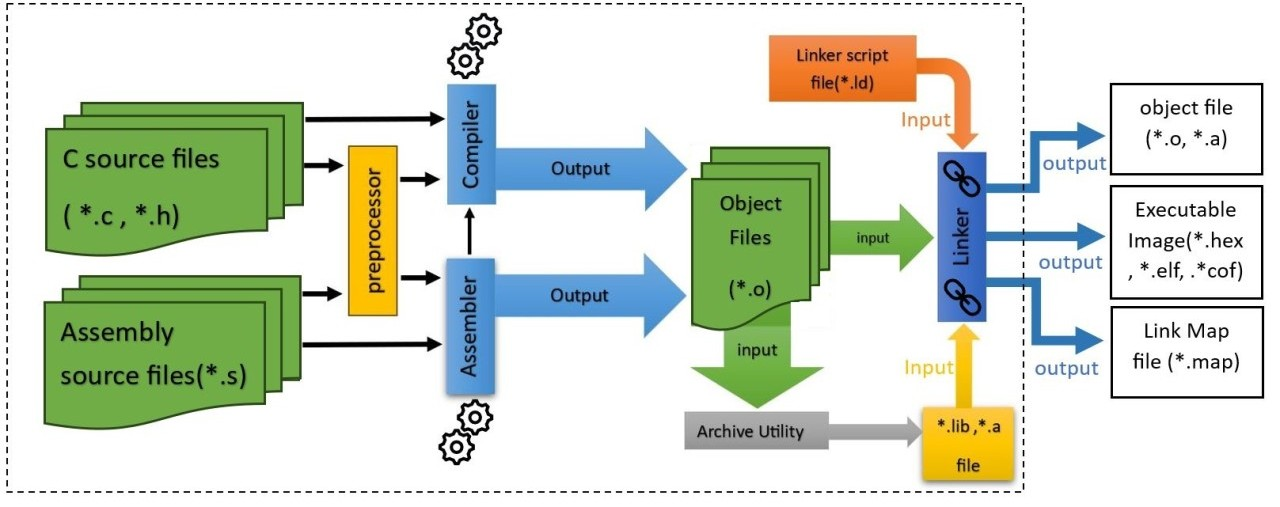
\includegraphics[width=15cm]{img/comp_diag.jpeg}
  \caption{Compilation Process Diagram}
  \label{fig:compilation}
\end{figure}
Going from source code in C/C++ to executable firmware involves multiple steps, in this subsection, we will go over them, highlighting the importance of each procedure.
\begin{itemize}
    \item \textbf{Preprocessor :} preprocessing is the first step of the build process, it expands macros and resolves defines as well as stripping comments from the code.
    \item \textbf{Assembler :} The assembler is the part of the toolchain that translates the high-level code into assembly code, which is the human-readable format of machine instruction.
    \item \textbf{Compiler :} Although the we use the term compilation as an equivalent to the whole process, compilation at its core is translating code into machine instructions, this step is what takes assembly mnemonics and turns them into machine code also known as object files.
    \item \textbf{Linker :} The linking stage is the final and most important part of the process, since every c file is compiled separately into its own object file, they are not executable by default, the linker is what declares memory regions and associates symbols to the appropriate sections.
\end{itemize}
\subsection{Embedded Systems Toolchains}
Building applications for embedded systems is quite different from a native build process, although you can create your own cross-compilation toolchain, there are available battle-tested available toolchains that are used across the industry. The most relevant ones being:
\begin{itemize}
    \item \textbf{GCC :} The GCC compiler is an open-source C/C++ compiler, and is part of the GNU utilities, ARM provides their own implementation, prefixed with "arm-none-eabi" and can target most ARM architectures such as ARMv7 and ARMv8.
    \item \textbf{ARM Compiler :} As well as providing a cross-compiling gcc toolchain, ARM has their own compiler based on CLANG and LLVM technologies called ARM compiler.
    \item \textbf{IAR Embedded Workbench:} IAR Systems is a Swedish computer software company that offers development tools for embedded systems. They are known for having a comprehensive development suite and an optimized compiler based on GCC.
\end{itemize}
\subsection{Build Runners}
Whereas simple projects can be compiled directly by invoking the corresponding command via an IDE or a terminal, as the project grows more complex, maintaining dependencies and flags becomes hard; that's where build runners or build system generators come in. They apply a rule-based mechanism to produce the desired output whether it be a library or an executable from its input which is the project's source code.
We find two main runners used:
\begin{itemize}
    \item \textbf{Make:} Make is a tool which controls the generation of executables and other non-source files of a program from the program's source files. Make is based on a file named "Makefile" at the top level of the project, it contains the necessary informations describing the build process and how to compute the desired output files.
    \item \textbf{Ninja:} Ninja is a small build system with a focus on speed. It differs from other build systems in two major respects: it is designed to have its input files generated by a higher-level build system, and it is designed to run builds as fast as possible.
\end{itemize}
\newpage
\subsection{CMake}
Although build runners alone work in a small scope, they do not provide enough flexibility to work across different environments or have multiple targets. This is the problem that CMake solves; it is a cross-platform build-system generator, that allows your project to run in different contexts without having to write platform specific configuration. It supports dependency management, integrates seamlessly with multiple IDEs and toolchains and offers builtin test and packaging support.
\section{Open-CMSIS-Pack}
Software compatibility for component re-use has long been a challenge in the microcontroller space, which is much more diverse at the hardware level compared to PCs or the data center. Open-CMSIS-Pack removes this complexity, delivering a standard for software component packaging and related foundation tools for validation, distribution, integration, management, and maintenance.
\subsection{CMSIS-Packs} CMSIS-Packs are software components that contain device specific startup code, peripheral drivers, middleware, and board support packages. They provide a standardized delivery mechanism for software components and enable consistent project configuration across different development environments.
\begin{figure}[H]
  \centering
  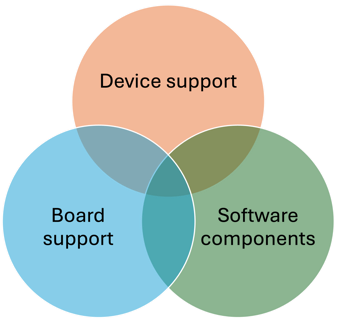
\includegraphics[height=10cm]{img/ST_Summer_Internship/pack_trinity.png}
  \caption{Software Packs Types}
  \label{fig:sw_trinity}
\end{figure}
\subsubsection{CMSIS-Pack Format}
The CMSIS-Pack format is used to deliver a software package and is aimed to be scalable for future requirements. It provides a management process and supports a tool independent distribution for:
\begin{itemize}
    \item \textbf{Device Support :}
    \begin{itemize}
        \item Information about the processor and it's features.
        \item C and assembly files for the device startup and access to the memory mapped peripheral registers.
        \item Parameters, technical information, and data sheets about the device family and the specific devices.
        \item Device description and available peripherals.
        \item Memory layout of internal and external RAM and ROM address ranges.
        \item Flash algorithms for programming the device.
        \item Debug and trace configurations as well as System View Description files for device specific display of the memory mapped peripheral registers. 
    \end{itemize}
    \item \textbf{Board Support :}
    \begin{itemize}
        \item Information about the development board and it's features.
        \item Parameters, technical information, and data sheets about the board, the mounted microcontroller, and peripheral devices.
        \item Drivers for on-board peripheral devices
    \end{itemize}
    \item \textbf{Software components :}
    \begin{itemize}
        \item A collection of source modules, header and configuration files as well as libraries.
        \item Documentation of the software, including features and APIs.
    \end{itemize}
\end{itemize}
\subsubsection{Software Components}
A software component encapsulates a set of related functions. They can contain C/C++ source files, object code, assembler files, header files, or libraries. The interfaces of software components should be defined with APIs to make them substitutable by other compatible components at design time.
CMSIS software components can also refer to multiple interfaces of other software components. This could be also a hardware abstraction layer for a device peripheral.
Configuration files contain application specific parameters for a software component. These files are typically copied to the user project workspace; all other files are not modified by the user and can remain in a separate location which avoids that a project workspace is polluted by many source files that should be considered as “black-box” elements by the application programmer.
\begin{figure}[H]
  \centering
  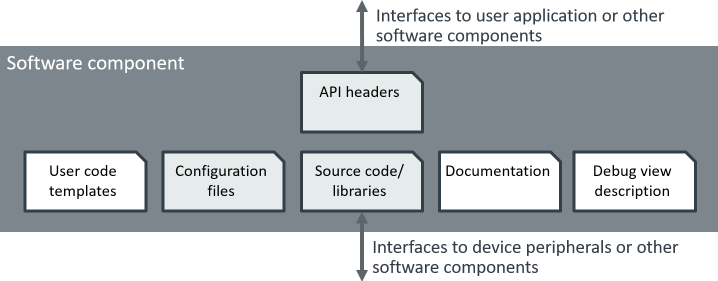
\includegraphics[width=15cm]{img/ST_Summer_Internship/software_component.png}
  \caption{Software Component Interface}
  \label{fig:sw_comp}
\end{figure}
\subsubsection{Component classification}
A component lists the files that belong to it and that are relevant for a project. The component itself or each individual file may refer to a condition that must resolve to true; if it is false, the component or file is not applicable in the given context.

Each software component must have the following attributes that are used to identify the component:
\begin{itemize}
    \item \textbf{Component Class (Cclass):} A component class which is a top-level component name, for example CMSIS, Device, File System
    \item \textbf{Component Group (Cgroup):} A component group name, for example CMSIS:RTOS, Device:Startup, File System:CORE
    \item \textbf{Component Version (Cversion):} the version number of the software component.
\end{itemize}



\subsection{CMSIS-Toolbox} The CMSIS-Toolbox provides command-line tools for project creation and build of embedded applications utilizing CMSIS-Packs. It supports multiple compilation tools. It also helps you with software pack creation, maintenance, and distribution utilizing the CMSIS-Pack format.
\subsubsection{Overall Workflow}
The CMSIS-Toolbox includes the following tools for the creation of embedded applications:
\begin{itemize}
    \item \textbf{ Pack Manager (cpackget):} install and manage software packs in the host development environment.
    \item \textbf{Project Manager (csolution):} create build information for embedded applications that consist of one or more related projects. It performs the following operations:
    \begin{itemize}
        \item \textbf{In the Project Area:} Generate build information files *.cbuild-idx.yml and *.cbuild.yml with all relevant project information for the build process.
        \item \textbf{In the RTE Directory:}
        \begin{itemize}
            \item Generate for each context the RTE\_components.h file and pre-include files from the software pack (*.pdsc) metadata.
            \item Copy the configuration files from selected software componentsand provide PLM information.
        \end{itemize}
    \end{itemize}
    \begin{figure}[H]
      \centering
      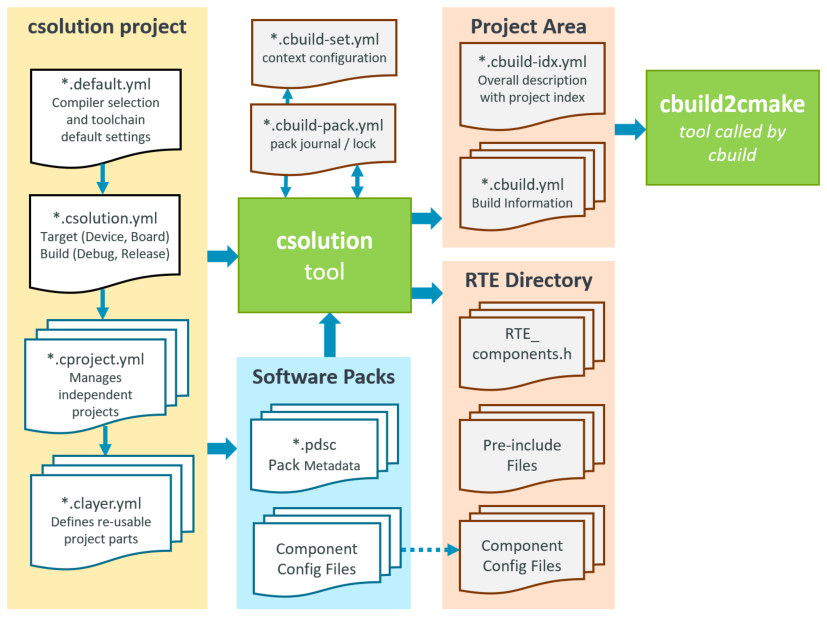
\includegraphics[width=15cm]{img/ST_Summer_Internship/csolution-operation.png}
      \caption{Csolution Operation}
      \label{fig:csolution_op}
    \end{figure}    
    \item \textbf{Build Invocation (cbuild):} orchestrate the build steps utilizing CMSIS tools and a CMake compilation process. It has two overall modes :
    \begin{itemize}
        \item \textbf{build mode:} generates the application and is the default command.
        \begin{itemize}
            \item When option --packs is used, it downloads missing software packs using cpackget.
            \item It calls csolution to process the the <name>.csolution.yml project. The output are build information files with all relevant project information for the build process.
        \end{itemize}
        \item  \textbf{setup mode:} generates the setup information for an IDE to populate dialogues, IntelliSense, and project outline views.
        \begin{itemize}
            \item Check YML file syntax against schema for all files specified by *.csolution.yml.
            \item Check the correctness of all files specified by *.csolution.yml.
        \end{itemize}
    \end{itemize}
    \begin{figure}[H]
      \centering
      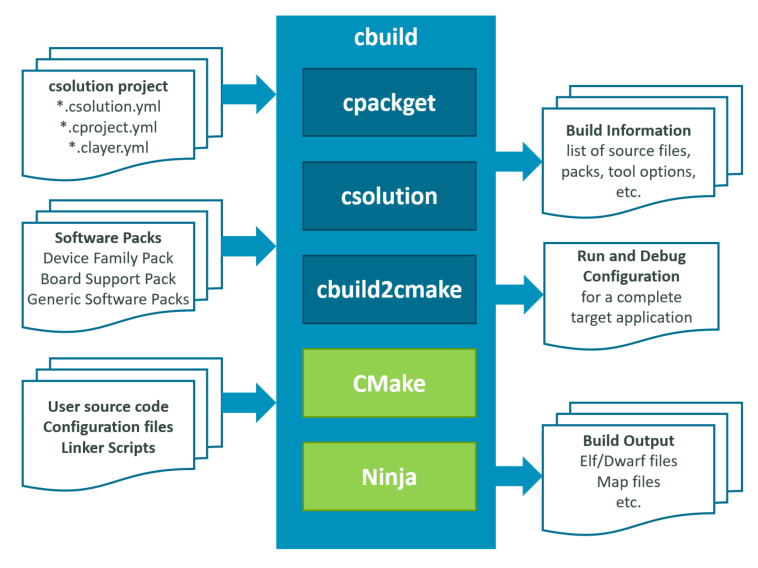
\includegraphics[width=15cm]{img/ST_Summer_Internship/cbuild-workflow.png}
      \caption{Cbuild Workflow}
      \label{fig:cbuild_wf}
    \end{figure}
\end{itemize}
\subsubsection{CMSIS solution files}
The CMSIS-Toolbox gets its information from the csolution project files, these are YAML configuration files used to describe the application's context:
\begin{itemize}
    \item \textbf{Solution file} A solution is the software view of the complete system. It combines projects that can be generated independently and therefore, manages related projects. It also specifies the targeted device(s) and build type(s). The file has the format *.csolution.yml.
    \item \textbf{Project file} The *.cproject.yml file has the content of a single independent build step, it specifies the source files to compile, sets the include directories and the necessary defines.
    \item \textbf{Layer file} Software layers collect source files and software components along with configuration files for reuse in different projects. Software Layers gives projects a better structure and simplifies:
    \begin{itemize}
        \item Development flows with evaluation boards and production hardware.
        \item Evaluation of middleware and hardware modules across different microcontroller boards.
        \item Code reuse across projects, i.e. board support for test-case deployment.
        \item Test-driven software development on simulation model and hardware.
    \end{itemize}
    \item \textbf{Default Configuration file} The cdefault.yml file contains a common set of compiler-specific settings that select reasonable defaults with miscellaneous controls for each compiler. 
\end{itemize}
\subsubsection{Cbuild2cmake}
cbuild2cmake reads the build information files *.cbuild-idx.yml and *.cbuild.yml to get all relevant project information for the build process. It generates the  output files for CMake build system; describing the overall application build process with the current context configuration, as well as the toolchain specific configuration and source file definitions for groups and software components. CMake is then invoked twice.
\begin{itemize}
    \item
    CMake configuration command defines the build generator, source, and build directory with:
    \begin{lstlisting}
        cmake -G Ninja -S <tmpdir> -B <tmpdir> -Wnodev
    \end{lstlisting}
    \item
    CMake build command to build the application program for each context with:
    \begin{lstlisting}
        cmake --build <tmpdir> -j <n> --target <context>
    \end{lstlisting}
\end{itemize}

\section{Project Generation}
When trying to run benchmarks across a wide variety of MCUs, the project structure follows the same pattern, and the dependencies can be expressed in a logical way relating to the device's metadata.
Therefore, automating the process will prove handy since every single step can be automated.
There are multiple techniques to be used to generate a fully working project from scratch.
\subsection{Regular Expressions:}
    The phrase regular expressions, or regexes, is often used to mean the specific, standard textual syntax for representing patterns for matching text. Each character in a regular expression (that is, each character in the string describing its pattern) is either a metacharacter, having a special meaning, or a regular character that has a literal meaning.
    A regular expression, often called a pattern, specifies a set of strings required for a particular purpose. 
\subsubsection{Operations}
Most formalisms provide the following operations to construct regular expressions. 
\begin{itemize}
    \item \textbf{Boolean "OR":} A vertical bar separates alternatives. For example, gray|grey can match "gray" or "grey".
    \item \textbf{Grouping} Parentheses are used to define the scope and precedence of the operators (among other uses). For example, gray|grey and gr(a|e)y are equivalent patterns which both describe the set of "gray" or "grey".
    \item \textbf{Quantification} A quantifier after an element (such as a token, character, or group) specifies how many times the preceding element is allowed to repeat.
    The available quantifications are:
    \begin{itemize}
        \item \textbf{Zero or One:} Denoted by the question mark \textbf{"?"} symbol.
        \item \textbf{Zero or More:} Denoted by the asterisk \textbf{"*"} (derived from the Kleene star). 
        \item \textbf{One or More:} Denoted by the plus symbol \textbf{"+"}.
        \item \textbf{N or More:} Denoted by the expression : \textbf{"\{N, \}"} where N is a positive integer.
        \item \textbf{N or Less:} Denoted by the expression : \textbf{"\{ ,N\}"} where N is a positive integer.
        \item \textbf{Between N and M times:} Denoted by the expression: \textbf{"\{N, M\}"} where N and M are positive integers such that N < M.
    \end{itemize}
    \item \textbf{Wildcard:} Denoted by the dot \textbf{"."} it matches any single character
\end{itemize}
These operations can be combined interchangeably to create complex expressions to describe the desired system.
\subsubsection{IEEE POSIX Standard}
The IEEE POSIX standard has three sets of compliance: BRE (Basic Regular Expressions), ERE (Extended Regular Expressions), and SRE (Simple Regular Expressions). SRE is deprecated, in favor of BRE, as both provide backward compatibility.
BRE and ERE work together. ERE adds ?, +, and |, and it removes the need to escape the metacharacters ( ) and \{ \}, which are required in BRE. Furthermore, as long as the POSIX standard syntax for regexes is adhered to, there can be, and often is, additional syntax to serve specific (yet POSIX compliant) applications. Although POSIX.2 leaves some implementation specifics undefined, BRE and ERE provide a "standard" which has since been adopted as the default syntax of many tools, where the choice of BRE or ERE modes is usually a supported option.
Perl regexes have become a de facto standard, having a rich and powerful set of atomic expressions. Perl has no "basic" or "extended" levels. As in POSIX EREs, ( ) and \{ \} are treated as metacharacters unless escaped; other metacharacters are known to be literal or symbolic based on context alone. Additional functionality includes lazy matching, backreferences, named capture groups, and recursive patterns.

\subsection{Templates \& File Manipulation}
File generation templates are pre-defined structures or blueprints used to create new files with standardized content and formatting.
\subsubsection{Template Definition}
A template file is created containing boilerplate text, placeholders for dynamic content (variables), and sometimes logic for conditional generation.
\subsubsection{Parameterization}
The template defines parameters that can be filled in by the user or a program when generating a new file. These parameters can include names, dates, specific values, or other relevant information.
\subsubsection{Template Execution}
When a new file is needed, the template is selected, and the required parameters are provided. A generation engine then processes the template, replacing placeholders with the provided values and executing any embedded logic to produce the final file.
\begin{figure}[H]
	\centering
	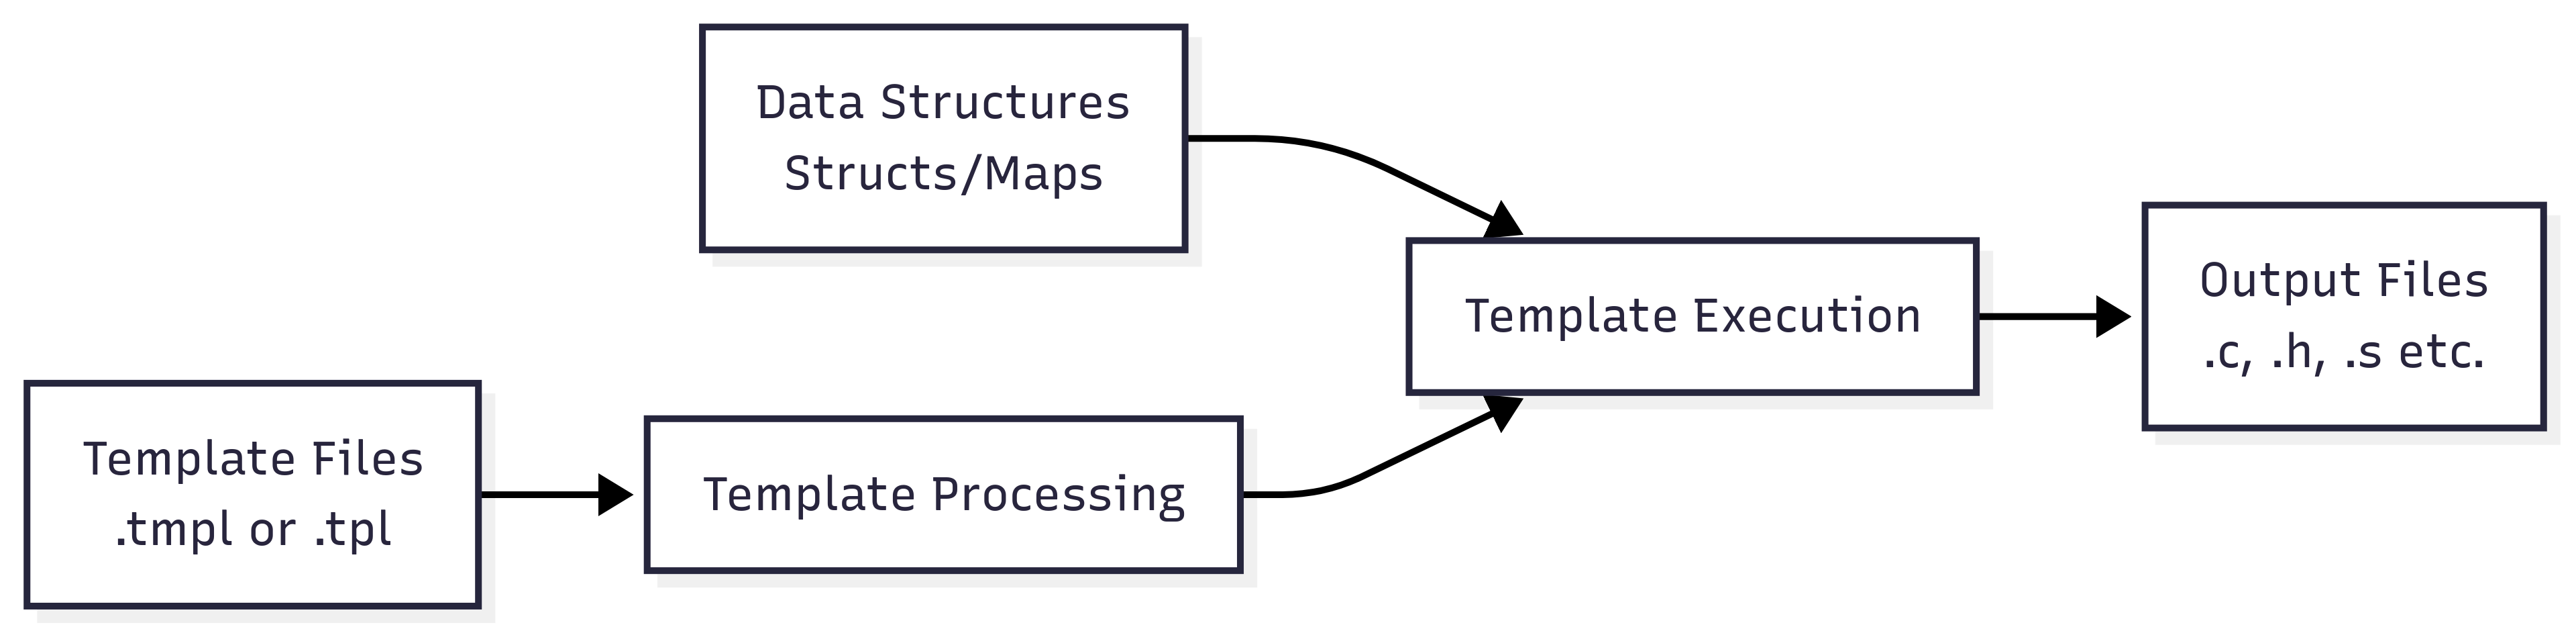
\includegraphics[width=15cm]{img/ST_Summer_Internship/template_workflow.png}
	\caption{Templating Process}
	\label{fig:tempalte_proc}
\end{figure}

\subsection{CMSIS-Toolbox Generators}
Generators, such as STM32CubeMX or MCUXpresso Config Tools, simplify the configuration for devices and boards. The CMSIS-Toolbox implements a generic interface for generators. They may be used to:
\begin{itemize}
	\item Configure device and/or board settings, such as clock configuration or pinout.
	\item Add and configure software drivers, for example, for UART, SPI, or I/O ports.
	\item Configure parameters of an algorithm, such as DSP filter design or motor control parameters.
\end{itemize}
\subsubsection{Generator Integration (STM32CubeMX Example)}
\begin{figure}[H]
	\centering
	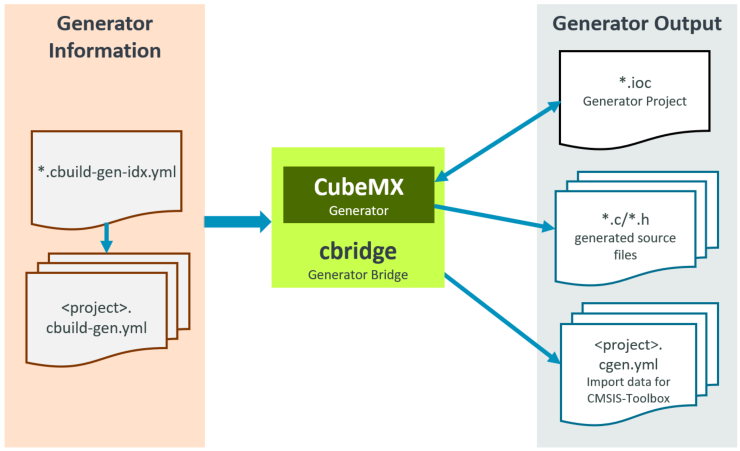
\includegraphics[width=15cm]{img/Generator-Integration.png}
	\caption{Generator Integration in CMSIS-Toolbox}
	\label{fig:generator}
\end{figure}
The Figure \ref{fig:generator} shows how the STM32CubeMX generator is integrated into the CMSIS build process. The data flow is exemplified on STM32CubeMX (Generator ID for this example is CubeMX). The information about the project is delivered to the generator using the Generator Information files (<solution-name>.cbuild-gen-idx.yml and <context>.cbuild-gen.yml). This information provides CubeMX with the project context, such as the selected board or device, and CPU mode, such as TrustZone, disabled/enabled.
The utility cbridge gets as parameter the <solution-name>.cbuild-gen-idx.yml and calls the generator. For the CubeMX generator example, these files are created:
\begin{itemize}
	\item *.ioc CubeMX project file with current project settings
	\item *.c/.h source files, i.e. for interfacing with drivers
	\item <project-name>.cgen.yml (created by cbridge) provides the data for project import into the csolution build process.
\end{itemize}
\newpage
\section{Loading And Debugging}
Within the context of this project, there are two different approaches to running our application, we will explore both of them providing insight on the advantages of limitations of both.
\subsection{PyOCD}
In the ideal usecase, \textbf{PyOCD} offers all the needed tools to run and debug our application.
\begin{figure}[H]
    \centering
    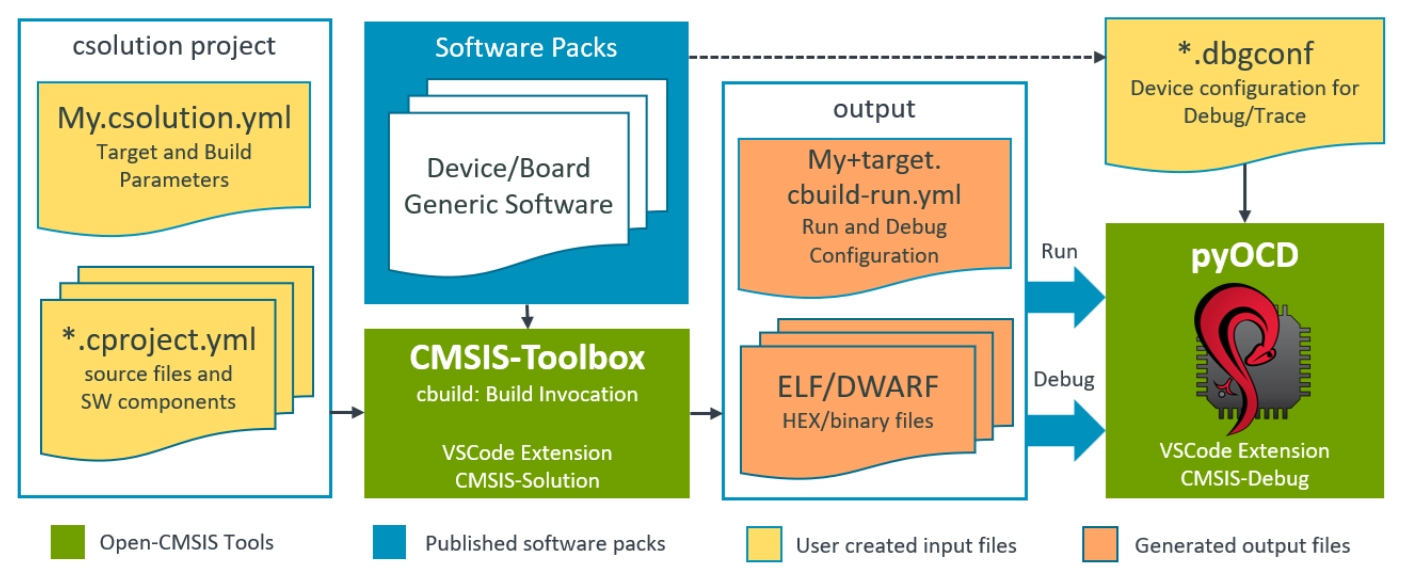
\includegraphics[width=15cm]{img/ST_Summer_Internship/cbuild-run.png}
    \caption{PyOCD Running and Debugging Workflow}
    \label{fig:debug_wf}
\end{figure}
The CMSIS-Toolbox build system manages software packs that contain information about device, board, and software components. It controls the build output (typically ELF/DWARF files), and has provisions for HEX, BIN and post-processing.
\subsubsection*{Configuration \& Settings}
The CMSIS-Toolbox uses the information from the DFP and BSP to simplify the debugger configuration. It generates the file *.cbuild-run.yml that contains for one target of a csolution project all information for run and debug.
The software packs contain information that is the basis for debug and run settings:
\begin{itemize}
    \item Flash algorithms of device memory (in DFP) and board memory (in BSP).
    \item On-board debug adapter (a default programming/debug channel) including features.
    \item Available memory of device and board.
    \item Device parameters such as processor core(s) and clock speed.
    \item Debug Access Sequences and System Description Files that support more complex Cortex-A/R/M configurations.
    \item Debug Configuration files (*.dbgconf) that configure device properties such as trace pins.
    \item CMSIS-SVD SVD files for viewing device peripherals.
    \item CMSIS-View SCVD files for analysis of software components (RTOS, Middleware).
\end{itemize}
\subsection{STM32CubeProgrammer}
While more convenient, PyOCD relies on recognizing the connected device in order to perform its operations, while for commercialized devices, this works fine. When working on products that have not been launched, or better yet, still in the pre-production phase, only available as a prototype running on an FPGA, PyOCD no longer can serve its purpose.
That's where \textbf{STM32CubeProgrammer} comes into play, since the tool is developed within the premises of \textbf{ST}, we are able to load our program into all STM32 MCUs.
\section*{Conclusion}
This chapter provided the foundational knowledge required to understand the subsequent work in this report. We began by exploring the STM32 ecosystem, examining the wide range of available microcontrollers, their ARM Cortex-M cores, and critical peripherals such as UART. We also reviewed the STM32Cube firmware package, which streamlines development through standardized libraries like CMSIS, HAL, and LL drivers.

Next, we covered benchmarking principles with a focus on embedded systems. We highlighted the unique challenges of benchmarking microcontrollers, including clock source provisioning, memory mapping, and custom I/O implementations. CoreMark was introduced as a reliable and widely adopted benchmark for evaluating MCU performance in a standardized manner, providing meaningful metrics for comparison.

Afterwards, we discussed the embedded systems build process, emphasizing the importance of toolchains, linking, and memory management. We examined build systems like Make, Ninja, and CMake as a higher-level generator for complex, cross-platform builds.

A key part of this chapter was the introduction of Open-CMSIS-Pack and the CMSIS-Toolbox, which address the complexity of managing device- and board-specific software components. We detailed their role in packaging, versioning, and automating builds.

Finally, we explored project generation techniques, from basic methods like regular expressions and templating to advanced integration with generators like STM32CubeMX.

In summary, this chapter established a comprehensive theoretical framework, connecting concepts of hardware, benchmarking, toolchains, and automation. These concepts form the backbone of the methodology applied in later chapters, ensuring that the processes for benchmarking and project generation are both systematic and scalable.
